\documentclass{beamer}



\usepackage{xcolor}
\usepackage{tikz}
\usetikzlibrary{arrows,decorations.pathmorphing,positioning,fit,trees,shapes}



\title{Difference Logic \\
    {\large Satisfiability Checking Seminar}
}
\author{Alex Ryndin \\ Supervisor: Gereon Kremer}
\date{WS 2016/2017}



\begin{document}
    \maketitle



    \begin{frame}
        \frametitle{Outline}
        \begin{itemize}
            \item Main Literature
            \item Difference Logic and Why It Is Important
            \item SAT Checking of Propositional Logic
            \item SAT Checking of Difference Logic
            \item Constraint Graph
            \item Negative Cycles in a Constraint Graph
            \item How to Find a Negative Cycle in a Graph
            \item Conclusion
        \end{itemize}
    \end{frame}



    \begin{frame}
        \frametitle{Main Literature}
        \begin{itemize}
            \item Scott Cotton, Eugene Asarin, Oded Maler
            and Peter Niebert. \textbf{``Some progress in
            satisfiability checking for difference logic``}.
            In Formal Techniques, Modelling and Analysis
            of Timed and Fault-Tolerant Systems,
            pages 263--276. Springer, 2004.
            \item Andrew V. Goldberg and Tomasz Radzik.
            \textbf{``A heuristic improvement of the Bellman-Ford
                algorithm``}.
            Applied Mathematics Letters, 6(3):3–6, 1993.
            \item Thomas H. Cormen, Charles E. Leiserson,
            Ronald L. Rivest and Clifford Stein.
            \textbf{``Introduction to algorithms``}.
            MIT press, third edition, 2009.
            \\
            Note: the chapter 24
            \textbf{``Single-Source Shortest Paths``}
            is relevant for the topic.
        \end{itemize}
    \end{frame}



    \begin{frame}
        \frametitle{Difference Logic and Why It Is Important}
        \begin{itemize}
            \item Difference logic (DL) is a special case of
            linear arithmetic (LA) logic.
            \item It is a Propositional Logic (PL)
            enhanced with constraints of the following form:
            \begin{equation}
                x - y \prec c
            \end{equation}
            where $ x,y $ are variables, $ c $ is a constant
            and $ \prec \in \{ <, \le \} $ is a comparison operator.
            \item $ x,y,c $ can be defined either over
            Integers $ \mathbb{Z} $
            or over Reals $ \mathbb{R} $.
        \end{itemize}
    \end{frame}




    \begin{frame}
        \frametitle{Difference Logic and Why It Is Important}
        \begin{itemize}
            \item A couple of examples:
        \end{itemize}
        \begin{equation}
            \phi_1 = (p \lor q)
            \land (p \rightarrow (u - v < 3.3))
            \land (q \rightarrow (v - w < -5.15))
        \end{equation}
        \begin{equation}
            \begin{aligned}
                \phi_2 &= (u-v < 1) \land (v-w < 5) \\
                & \land (w-x \leq -3) \land (x-y < 1) \\
                & \land (y-z \leq -5) \land (y-v \leq 0) \\
            \end{aligned}
        \end{equation}
        \begin{equation}
            \begin{aligned}
                \phi_3 &= (u-v < 1) \land (v-w < 5) \\
                & \land (w-x \leq -3) \land (x-y < -3) \\
                & \land (y-z \leq -5) \land (y-w < 4) \\
            \end{aligned}
        \end{equation}
    \end{frame}



    \begin{frame}
        \frametitle{Scheduling Problem Example}
        \begin{figure}[htb]
            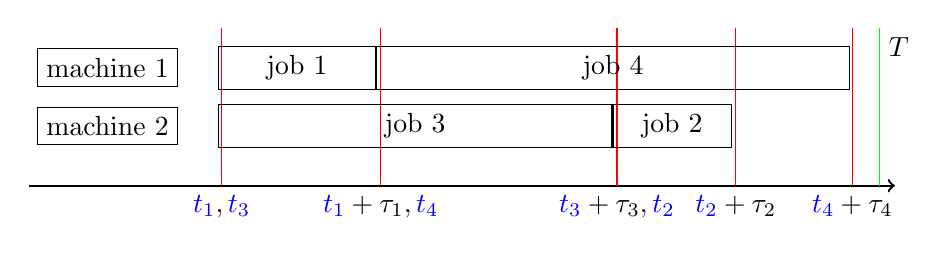
\begin{tikzpicture}
                \draw[thick,->] (-1,-1.5) -- (10,-1.5);

                \draw[color=red] (1.45,0.5) -- (1.45,-1.5);
                \draw (1.45,-1.5) -- (1.45,-1.5)
                            node[anchor=north] {$ \textcolor{blue}{t_1}, \textcolor{blue}{t_3} $};

                \draw[color=red] (3.47,0.5) -- (3.47,-1.5);
                \draw (3.47,-1.5) -- (3.47,-1.5)
                            node[anchor=north] {$ \textcolor{blue}{t_1}+\tau_1, \textcolor{blue}{t_4} $};

                \draw[color=red] (6.47,0.5) -- (6.47,-1.5);
                \draw (6.47,-1.5) -- (6.47,-1.5)
                            node[anchor=north] {$ \textcolor{blue}{t_3}+\tau_3, \textcolor{blue}{t_2} $};

                \draw[color=red] (7.98,0.5) -- (7.98,-1.5);
                \draw (7.98,-1.5) -- (7.98,-1.5)
                            node[anchor=north] {$ \textcolor{blue}{t_2}+\tau_2 $};

                \draw[color=red] (9.46,0.5) -- (9.46,-1.5);
                \draw (9.46,-1.5) -- (9.46,-1.5)
                            node[anchor=north] {$ \textcolor{blue}{t_4}+\tau_4 $};

                \draw[color=green] (9.8,0.5) -- (9.8,-1.5);
                \draw (9.8,0.5) -- (9.8,0.5)
                            node[anchor=north west] {$ T $};

                \node [draw] (m1) at (0,0) {machine 1};
                \node [draw, below = 0.25cm of m1] (m2) {machine 2};
                \node [draw, minimum width=2cm,
                        right = 0.5cm of m1]
                                        (job1) {job 1};
                \node [draw, minimum width=6cm,
                        right = 0cm of job1]
                                        (job4) {job 4};
                \node [draw, minimum width=5cm,
                        right = 0.5cm of m2]
                                        (job3) {job 3};
                \node [draw, minimum width=1.5cm,
                        right = 0cm of job3]
                                        (job2) {job 2};
            \end{tikzpicture}
        \end{figure}
    \begin{itemize}
        \item $ \textcolor{blue}{p_{mj}} = True $
        if job $ j $ is scheduled
        on machine $ m $:
        \\
        e.g. $ \textcolor{blue}{p_{11}} = \textcolor{blue}{p_{14}} = \textcolor{blue}{p_{23}} = \textcolor{blue}{p_{22}} = True $
        for the figure above
        \item job $ i $ starts at $ \textcolor{blue}{t_i} $
        and lasts $ \tau_i $
        \item a machine cannot process two or more jobs
        simultaneously:
        \\
        $ (\textcolor{blue}{p_{mi}} \land \textcolor{blue}{p_{mj}}) \rightarrow ((\textcolor{blue}{t_i} + \tau_i \le \textcolor{blue}{t_j}) \lor (\textcolor{blue}{t_j} + \tau_j \le \textcolor{blue}{t_i})) \quad \Leftrightarrow $
        \\
        $ (\textcolor{blue}{p_{mi}} \land \textcolor{blue}{p_{mj}}) \rightarrow ((\textcolor{blue}{t_i} - \textcolor{blue}{t_j} \le -\tau_i) \lor (\textcolor{blue}{t_j} - \textcolor{blue}{t_i} \le -\tau_j)) $
        \item the overall processing time should not exceed $ T $:
        \\
        $ \textcolor{blue}{t_i} + \tau_i \le T \quad \Leftrightarrow \quad \textcolor{blue}{t_i} - 0 \le T -\tau_i $
    \end{itemize}
    \end{frame}



    \begin{frame}
        \frametitle{Scheduling Problem Example}
        \begin{equation*}
            \begin{aligned}
                \phi &= \bigwedge_{j=1}^{4} (p_{1j} \lor p_{2j}) \quad \land \\
                & \mathrm{each \; task \; is \; executed \; on \; at \; least \; one \; machine} \\
                & \bigwedge_{j=1}^{4} ((p_{1j} \rightarrow \neg p_{2j}) \land (p_{2j} \rightarrow \neg p_{1j})) \quad \land \\
                & \mathrm{each \; task \; can \; be \; scheduled \; on \; one \; machine\; only } \\
                & \bigwedge_{j=1}^{4} (t_j \ge 0) \; \land \; \bigwedge_{j=1}^{4} (t_j \le T-\tau_j) \quad \land \\
                & \mathrm{general \; time \; constraints} \\
                & \bigwedge_{m=1}^{2} \bigwedge_{i=1}^{3} \bigwedge_{j=i+1}^{4} ((p_{mi} \land p_{mj}) \rightarrow ((t_i-t_j \le -\tau_i) \lor (t_j-t_i \le -\tau_j))) \\
                & \mathrm{no \; time \; overlap \; rule} \\
            \end{aligned}
        \end{equation*}
    \end{frame}



    \begin{frame}
        \frametitle{SAT Checking of Propositional Logic}
        ttt
    \end{frame}



    \begin{frame}
        \frametitle{SAT Checking of Difference Logic}
        ttt
    \end{frame}



    \begin{frame}
        \frametitle{Constraint Graph}
        ttt
    \end{frame}
    
    
    
    \begin{frame}
        \frametitle{Negative Cycles in a Constraint Graph}
        ttt
    \end{frame}
    
    
    
    \begin{frame}
        \frametitle{How to Find a Negative Cycle in a Graph}
        ttt
    \end{frame}



    \begin{frame}
        \frametitle{Conclusion}
        \begin{itemize}
            \item a
            \item b
            \item c
        \end{itemize}
    \end{frame}



    \begin{frame}
        \frametitle{Thank you}
        \Huge Thank you for your attention
    \end{frame}
\end{document}